\documentclass[12pt]{article}
\usepackage[english]{babel}
\usepackage{natbib}
\usepackage{url}
\usepackage[utf8x]{inputenc}
\usepackage{amsmath}
\usepackage{graphicx}
\graphicspath{{../docs/img/}}
\usepackage{parskip}
\usepackage{fancyhdr}
\usepackage{vmargin}
\usepackage{xcolor}
\usepackage{booktabs}
\usepackage{float}
\usepackage{pgfplots}
\usepackage{tikz}
\pgfplotsset{width=10cm,compat=1.9}

\setmarginsrb{3 cm}{2.5 cm}{3 cm}{2.5 cm}{1 cm}{1.5 cm}{1 cm}{1.5 cm}

\title{Sprint 4 Backlog}								% Title
\author{Thierry's Minions}								% Author
\date{12 Nov 2018}											% Date

\makeatletter
\let\thetitle\@title
\let\theauthor\@author
\let\thedate\@date
\makeatother

\pagestyle{fancy}
\fancyhf{}
\rhead{\theauthor}
\lhead{\thetitle}
\cfoot{\thepage}

\newcommand*{\userstory}[5][.25em]{
%  \begin{tabular*}{\maincolumnwidth}{l@{\extracolsep{\fill}}r}%
%    {\bfseries #2} & {\bfseries #4}\\%
%    {#3}\\%
%  \end{tabular*}%
%  \ifx&#5&%
%  \else{\\%
%    \begin{minipage}{\maincolumnwidth}%
%      #5%
%    \end{minipage}}\fi%
%  \par\addvspace{#1}
\textbf{#1} 
  }

\newcommand{\roundpic}[4][]{
  \tikz\node [circle, minimum width = #2,
    path picture = {
      \node [#1] at (path picture bounding box.center) {
        \includegraphics[width=#3]{#4}};
    }] {};}

\begin{document}

%%%%%%%%%%%%%%%%%%%%%%%%%%%%%%%%%%%%%%%%%%%%%%%%%%%%%%%%%%%%%%%%%%%%%%%%%%%%%%%%%%%%%%%%%

\begin{titlepage}
	\centering
    \vspace*{0.5 cm}
\roundpic[]{9cm}{9cm}{leader.jpg}

    \textsc{\LARGE Thierry's Minions/Team25\\[0.5em] Deliverable 4}\\[2.0 cm]	
	\textsc{\Large CSCC01 Fall 2018}\\[0.5 cm]				% Course Code
	\rule{\linewidth}{0.2 mm} \\[0.4 cm]
	{ \huge \bfseries \thetitle}\\
	\rule{\linewidth}{0.2 mm} \\[1.5 cm]
	
	\begin{minipage}{0.4\textwidth}
		\begin{flushleft} \large
			\emph{Submitted To:}\\
			Saba Kiaei\\
            Teaching Assistant\\
            Computer Science Department\\
			\end{flushleft}
			\end{minipage}~
			\begin{minipage}{0.4\textwidth}
            
			\begin{flushright} \large
			\emph{Submitted By :} \\
			Rishabh Kaant Sharma\\
            Joseph Sokolon\\
            Balaji Badu\\
            Jayden Arquelada\\
            Edgar Sarkisian\\
		\end{flushright}
        
	\end{minipage}\\[2 cm]
	
	
    
    
    
    
	
\end{titlepage}

%%%%%%%%%%%%%%%%%%%%%%%%%%%%%%%%%%%%%%%%%%%%%%%%%%%%%%%%%%%%%%%%%%%%%%%%%%%%%%%%%%%%%%%%%

\textcolor{black}{\tableofcontents}
\pagebreak

%%%%%%%%%%%%%%%%%%%%%%%%%%%%%%%%%%%%%%%%%%%%%%%%%%%%%%%%%%%%%%%%%%%%%%%%%%%%%%%%%%%%%%%%%

\section{Sprint Tasks}

\subsection{Task 3A: Create formatting functions}
\begin{itemize}%
\item Story Points: 2
\item Build formatting functions on the client that turn the data into consistent formats 
\item Phone numbers should all be made into format: XXX-XXX-XXXX
\item Postal code should all be made into format: XXXXXX
\item Dates should all be made into format: YYYY-MM-DD
\item Should throw an error if the data cannot be formatted.
\end{itemize}

\subsection{Task 3B: Format data}
\begin{itemize}%
\item Story Points: 3
\item This task has a dependency on task 3A
\item When parsing data should pass strings into formatting functions created in 3A
\item If formatter throws an error then should add column name into an array called invalidcolumns, and set valid to false.
\end{itemize}

\subsection{Task 5A: Create UI for Generate Simple Reports Screen}
\begin{itemize}%
\item Story Points: 3
\item Create a screen with 2 buttons.
\item One button for each report type. 
\item Connect screen to project via navigation bar.
\end{itemize}

\subsection{Task 5B: Create Controllers to send request to the server.}
\begin{itemize}%
\item Story Points: 3
\item Create a controller that makes a request to the server for data.
\item This data will be used to generate the report. 
\end{itemize}

\subsection{Task 5C: Create Controllers to send request to the server.}
\begin{itemize}%
\item Story Points: 5
\item Create a POST endpoint on the server to query the database and collect the data that will be sent back to client.
\item Body of the request will contain columns that client wants information on. 
\item Endpoint of the request will be /reports/get-data/.
\end{itemize}

\subsection{Task 5D: Generate Empty Report.}
\begin{itemize}%
\item Story Points: 5
\item Generate a empty report. 
\item Probably use Alpache PDF Library.
\item The report should be generated in the format of a PDF.
\item The report should contain a header and a configurable title.
\end{itemize}

\subsection{Task 5E: Generate Pie Chart for Report.}
\begin{itemize}%
\item Story Points: 5
\item This task has a dependency on task 5D
\item Generate a PIE Chart from data recieved from server.
\item Add the Chart to the PDF.
\end{itemize}

\subsection{Task 5F: Generate Pie Chart for Report.}
\begin{itemize}%
\item Story Points: 2
\item This task has a dependency on task 5D
\item Generate a Bar Chart from data recieved from server.
\item Add the Chart to the PDF.
\end{itemize}

\subsection{Task 5G: Generate Mock Data to Test Reporting.}
\begin{itemize}%
\item Story Points: 1
\item Fill in templates with mock data so we have a sizable quantitiy of data to display in the reports.
\end{itemize}

\subsection{Task 5H: Integrate and test feature.}
\begin{itemize}%
\item Story Points: 3
\item This task has a dependency on all previous tasks.
\item Ensure the integration between the server and client is working.
\item Test the entire feature and ensure it passes the conditions of acceptance.
\end{itemize}

\newpage
\section{Sprint Plan}

\textbf{Sprint 4 : November 3rd - November 9th (Saturday - Friday)}
\begin{table}[H]
\begin{tabular}{@{}c|c|c|c|ccccccc@{}}
\toprule
Story & Task & Dependency & \begin{tabular}[c]{@{}c@{}}Story\\ Points\end{tabular} & \begin{tabular}[c]{@{}c@{}}Day\\ 1\end{tabular} & \begin{tabular}[c]{@{}c@{}}Day\\ 2\end{tabular} & \begin{tabular}[c]{@{}c@{}}Day \\ 3\end{tabular} & \begin{tabular}[c]{@{}c@{}}Day \\ 4\end{tabular} & \begin{tabular}[c]{@{}c@{}}Day \\ 5\end{tabular} & \begin{tabular}[c]{@{}c@{}}Day \\ 6\end{tabular} & \begin{tabular}[c]{@{}c@{}}Day \\ 7\end{tabular} \\ \midrule
3     & A    &            & 2                                                      &                                                 & BB:2                                            &                                                  &                                                  &                                                  &                                                  &                                                  \\
3     & B    & A          & 3                                                      &                                                 &                                                 &                                                  &                                                  &  ES:3                                            &                                                  &                                                  \\
5     & A    &            & 3                                                      &                                                 &                                                 & BB:2                                             & BB:1                                             &                                                  &                                                  &                                                  \\
5     & B    &            & 3                                                      &                                                 &                                                 &                                                  &                                                  &                                                  & RS:3                                             &                                                  \\
5     & C    &            & 5                                                      &                                                 & JA:2                                            & JA:3                                             &                                                  &                                                  &                                                  &                                                  \\
5     & D    &            & 5                                                      &                                                 &                                                 &                                                  & ES:5                                             &                                                  &                                                  &                                                  \\ 
5     & E    & D          & 5                                                      &                                                 &                                                 &                                                  &                                                  &  JS:5                                            &                                                  &                                                  \\ 
5     & F    & D          & 2                                                      &                                                 &                                                 &                                                  &                                                  &                                                  & JS:2                                             &                                                  \\ 
5     & G    &            & 1                                                      &                                                 &                                                 &                                                  &                                                  &                                                  & ES:1                                             &                                                  \\ 
5     & H    & ALL        & 3                                                      &                                                 &                                                 &                                                  &                                                  &                                                  &                                                  & JA:3                                             \\ \bottomrule
\end{tabular}
\end{table}

\begin{itemize}%
\item Estimated story points team can complete: 32
\item Balaji will complete task 3A by end of day 2.
\item Edgar will complete task 3B, and release feature by end of day 5.
\item Balaji will complete task 5A by end of day 4.
\item Rishabh will complete task 5B by end of day 6.
\item Jayden will complete task 5C by end of day 3.
\item Edgar will complete task 5D by end of day 4.
\item Joey will complete task 5E by end of day 5.
\item Joey will complete task 5F by end of day 6.
\item Edgar will complete task 5G by end of day 6.
\item Jayden will complete task 5H, and release feature by end of day 7.
\item The team believes they can complete User Story 3 by end of day 6, \& User Story 5 by end of the day 7. 
\end{itemize}

\newpage

\section{Sprint Report}

\textbf{Sprint 4 : November 3rd - November 9th (Saturday - Friday)}
\begin{table}[H]
\begin{tabular}{@{}c|c|c|c|ccccccc@{}}
\toprule
Story & Task & Dependency & \begin{tabular}[c]{@{}c@{}}Story\\ Points\end{tabular} & \begin{tabular}[c]{@{}c@{}}Day\\ 1\end{tabular} & \begin{tabular}[c]{@{}c@{}}Day\\ 2\end{tabular} & \begin{tabular}[c]{@{}c@{}}Day \\ 3\end{tabular} & \begin{tabular}[c]{@{}c@{}}Day \\ 4\end{tabular} & \begin{tabular}[c]{@{}c@{}}Day \\ 5\end{tabular} & \begin{tabular}[c]{@{}c@{}}Day \\ 6\end{tabular} & \begin{tabular}[c]{@{}c@{}}Day \\ 7\end{tabular} \\ \midrule
3     & A    &            & 2                                                      &                                                 &                                                 & BB:2                                             &                                                  &                                                  &                                                  &                                                  \\
3     & B    & A          & 3                                                      &                                                 &                                                 &                                                  &                                                  &  ES:3                                            &                                                  &                                                  \\
5     & A    &            & 3                                                      &                                                 &                                                 &                                                  &                                                  &                                                  & BB:3                                             &                                                  \\
5     & B    &            & 3                                                      &                                                 &                                                 &                                                  &                                                  &                                                  & RS:5                                             &                                                  \\
5     & C    & A          & 5                                                      &                                                 & JA:2                                            & JA:4                                             &                                                  &                                                  &                                                  &                                                  \\
5     & D    &            & 5                                                      &                                                 &                                                 &                                                  & ES:3                                             &                                                  &                                                  &                                                  \\ 
5     & E    & D          & 5                                                      &                                                 &                                                 &                                                  &                                                  &                                                  &                                                  &                                                  \\ 
5     & F    & D          & 2                                                      &                                                 &                                                 &                                                  &                                                  &                                                  &                                                  &                                                  \\ 
5     & G    &            & 1                                                      &                                                 &                                                 &                                                  &                                                  &                                                  &                                                  &                                                  \\ 
5     & H    & ALL        & 3                                                      &                                                 &                                                 &                                                  &                                                  &                                                  &                                                  &                                                  \\ \bottomrule
\end{tabular}
\end{table}

\begin{itemize}%
\item Actual story points burned: 21
\item Balaji completed task 5A on day 6 instead of 3.
\item Task 5C took Jayden an hour longer then expected.
\item Joey didn't complete task 5E \& 5F, They will be carried over to next sprint.
\item Edgar didn't complete task 5G. It will be carried over until next sprint.
\item Story 5 - Report Generation will be carried over to next sprint.
\item The team completed User Story 3 on day 6 of the sprint. 
\end{itemize}

\section{Sprint Burndown Chart}

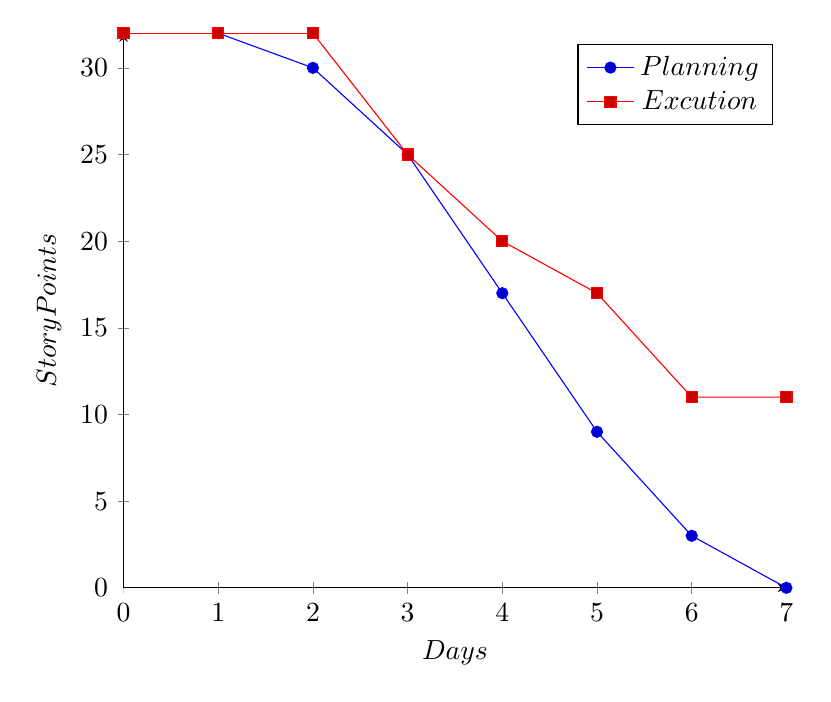
\begin{tikzpicture}
\begin{axis}[
    axis lines = left,
    xlabel = $Days$,
    ylabel = {$Story Points$},
]
\addplot coordinates {(0,32) (1,32) (2,30) (3,25) (4,17) (5,9) (6,3) (7,0)};
\addlegendentry{$Planning$}
\addplot coordinates {(0,32) (1,32) (2,32) (3,25) (4,20) (5,17) (6,11) (7,11)};
\addlegendentry{$Excution$}
\end{axis}
\end{tikzpicture}

\newpage
\bibliographystyle{plain}
\bibliography{biblist}

\end{document}